\documentclass[tikz,border=8pt]{standalone}
% Shared look for every TikZ diagram. Load with % Shared look for every TikZ diagram. Load with % Shared look for every TikZ diagram. Load with \input{../../tools/tikz-style.tex}
\usepackage[T1]{fontenc}
\usepackage{lmodern}
\renewcommand{\sfdefault}{lmr}  % diagrams use the same serif as the text
\usetikzlibrary{arrows.meta, positioning, shapes.geometric, calc, fit, backgrounds}
\definecolor{cblue}{HTML}{4C78A8}
\definecolor{corange}{HTML}{F58518}
\definecolor{cgreen}{HTML}{54A24B}
\definecolor{cred}{HTML}{E45756}
\definecolor{cpurple}{HTML}{B279A2}
\definecolor{cgrey}{HTML}{6B6B6B}
\tikzset{
  every picture/.style={font=\sffamily, line width=1.2pt},
  box/.style={draw=#1, fill=#1!12, rounded corners=4pt, align=center, inner sep=7pt, minimum height=1.1cm},
  box/.default=cgrey,
  arrow/.style={-{Stealth[length=3mm]}, draw=cgrey, line width=1.4pt},
  title/.style={font=\sffamily\bfseries\Large},
  note/.style={font=\sffamily\small, text=cgrey, align=center},
}
\AtBeginDocument{\hyphenpenalty=10000 \exhyphenpenalty=10000}

\usepackage[T1]{fontenc}
\usepackage{lmodern}
\renewcommand{\sfdefault}{lmr}  % diagrams use the same serif as the text
\usetikzlibrary{arrows.meta, positioning, shapes.geometric, calc, fit, backgrounds}
\definecolor{cblue}{HTML}{4C78A8}
\definecolor{corange}{HTML}{F58518}
\definecolor{cgreen}{HTML}{54A24B}
\definecolor{cred}{HTML}{E45756}
\definecolor{cpurple}{HTML}{B279A2}
\definecolor{cgrey}{HTML}{6B6B6B}
\tikzset{
  every picture/.style={font=\sffamily, line width=1.2pt},
  box/.style={draw=#1, fill=#1!12, rounded corners=4pt, align=center, inner sep=7pt, minimum height=1.1cm},
  box/.default=cgrey,
  arrow/.style={-{Stealth[length=3mm]}, draw=cgrey, line width=1.4pt},
  title/.style={font=\sffamily\bfseries\Large},
  note/.style={font=\sffamily\small, text=cgrey, align=center},
}
\AtBeginDocument{\hyphenpenalty=10000 \exhyphenpenalty=10000}

\usepackage[T1]{fontenc}
\usepackage{lmodern}
\renewcommand{\sfdefault}{lmr}  % diagrams use the same serif as the text
\usetikzlibrary{arrows.meta, positioning, shapes.geometric, calc, fit, backgrounds}
\definecolor{cblue}{HTML}{4C78A8}
\definecolor{corange}{HTML}{F58518}
\definecolor{cgreen}{HTML}{54A24B}
\definecolor{cred}{HTML}{E45756}
\definecolor{cpurple}{HTML}{B279A2}
\definecolor{cgrey}{HTML}{6B6B6B}
\tikzset{
  every picture/.style={font=\sffamily, line width=1.2pt},
  box/.style={draw=#1, fill=#1!12, rounded corners=4pt, align=center, inner sep=7pt, minimum height=1.1cm},
  box/.default=cgrey,
  arrow/.style={-{Stealth[length=3mm]}, draw=cgrey, line width=1.4pt},
  title/.style={font=\sffamily\bfseries\Large},
  note/.style={font=\sffamily\small, text=cgrey, align=center},
}
\AtBeginDocument{\hyphenpenalty=10000 \exhyphenpenalty=10000}

\usetikzlibrary{matrix}
\begin{document}
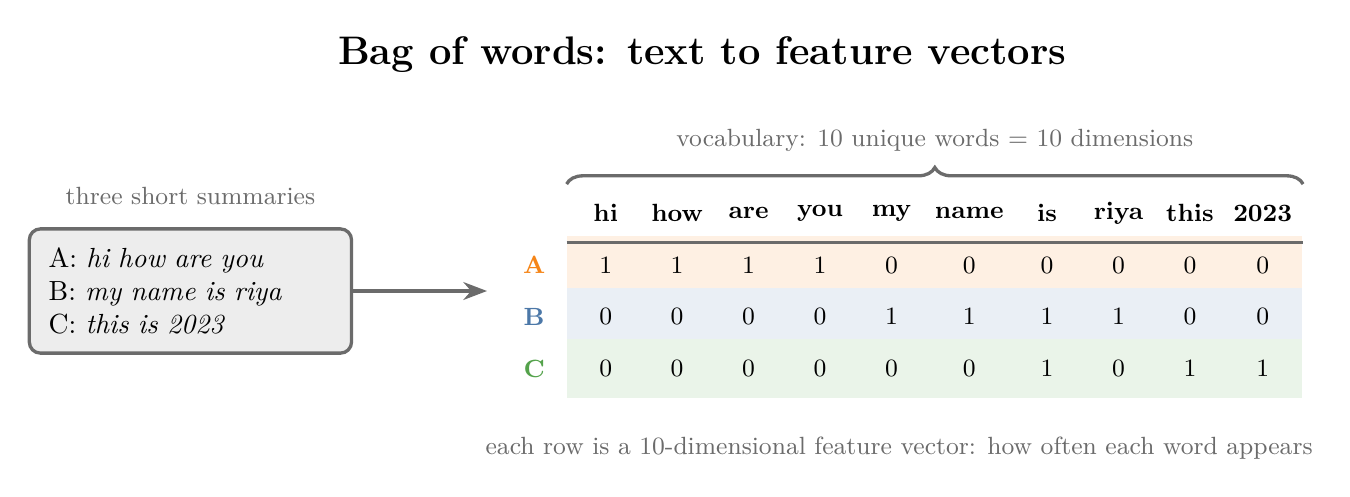
\begin{tikzpicture}
  \node[title] at (6.5,3.0) {Bag of words: text to feature vectors};
  % sentences
  \node[box=cgrey, text width=3.6cm, align=left] (s) at (0,0) {A: \textit{hi how are you}\\ B: \textit{my name is riya}\\ C: \textit{this is 2023}};
  \node[note, above=0.15cm of s] {three short summaries};
  % matrix
  \matrix (m) [matrix of nodes, nodes={minimum width=0.95cm, minimum height=0.7cm, font=\small, anchor=center},
               column sep=-\pgflinewidth, row sep=-\pgflinewidth] at (9,0) {
    |[font=\small\bfseries]| & |[font=\small\bfseries]| hi & |[font=\small\bfseries]| how & |[font=\small\bfseries]| are & |[font=\small\bfseries]| you & |[font=\small\bfseries]| my & |[font=\small\bfseries]| name & |[font=\small\bfseries]| is & |[font=\small\bfseries]| riya & |[font=\small\bfseries]| this & |[font=\small\bfseries]| 2023 \\
    |[font=\small\bfseries, text=corange]| A & 1 & 1 & 1 & 1 & 0 & 0 & 0 & 0 & 0 & 0 \\
    |[font=\small\bfseries, text=cblue]| B & 0 & 0 & 0 & 0 & 1 & 1 & 1 & 1 & 0 & 0 \\
    |[font=\small\bfseries, text=cgreen]| C & 0 & 0 & 0 & 0 & 0 & 0 & 1 & 0 & 1 & 1 \\
  };
  \begin{scope}[on background layer]
    \fill[corange!12] (m-2-2.north west) rectangle (m-2-11.south east);
    \fill[cblue!12] (m-3-2.north west) rectangle (m-3-11.south east);
    \fill[cgreen!12] (m-4-2.north west) rectangle (m-4-11.south east);
  \end{scope}
  \draw[cgrey, line width=0.8pt] (m-1-2.south west) -- (m-1-11.south east);
  \draw[decorate, decoration={brace, amplitude=6pt}, cgrey] (m-1-2.north west) -- (m-1-11.north east)
     node[midway, above=8pt, note] {vocabulary: 10 unique words = 10 dimensions};
  \draw[arrow] (s.east) -- ++(1.7,0);
  \node[note, below=0.25cm of m] {each row is a 10-dimensional feature vector: how often each word appears};
\end{tikzpicture}
\end{document}
